\subsection{Importer la librairie Java Phidgets dans Maven}
\begin{itemize}
\item Télécharger la documentation de la librairie à l’URL suivante :\\\url{http://www.phidgets.com/documentation/JavaDoc.zip}
\item Dézipper le fichier .zip télécharger et ouvrir un terminal dans le dossier résultant de dézippage
\item Lancer la commande \texttt{jar cf ../phidget-javadoc.jar}.
\item Télécharger la librairie Java de Phidgets à l’URL suivante : \url{http://www.phidgets.com/downloads/libraries/phidget21jar.zip}
\item Lancer la commande \texttt{mvn install:install-file -Dfile=phidget21.jar\\-DgroupId=com.phidgets -DartifactId=phidget -Dversion=2.1\\-Dpackaging=jar -Djavadoc=phidget-javadoc.jar} dans le dossier où se trouvent les .jar de la librairie et de la JavaDoc de celle-ci.
\item S'assurer que la dépendance suivante se trouve dans le pom.xml (ce qui est normalement déjà le cas) :
\begin{lstlisting}[language=XML, numbers=none]
<dependency>
    <groupId>com.phidgets</groupId>
    <artifactId>phidget</artifactId>
    <version>2.1</version>
    <scope>compile</scope>
</dependency>
\end{lstlisting}

\end{itemize}

\subsection{Photos de la maquette}

\begin{figure}[H]
    \begin{center}
        \frame{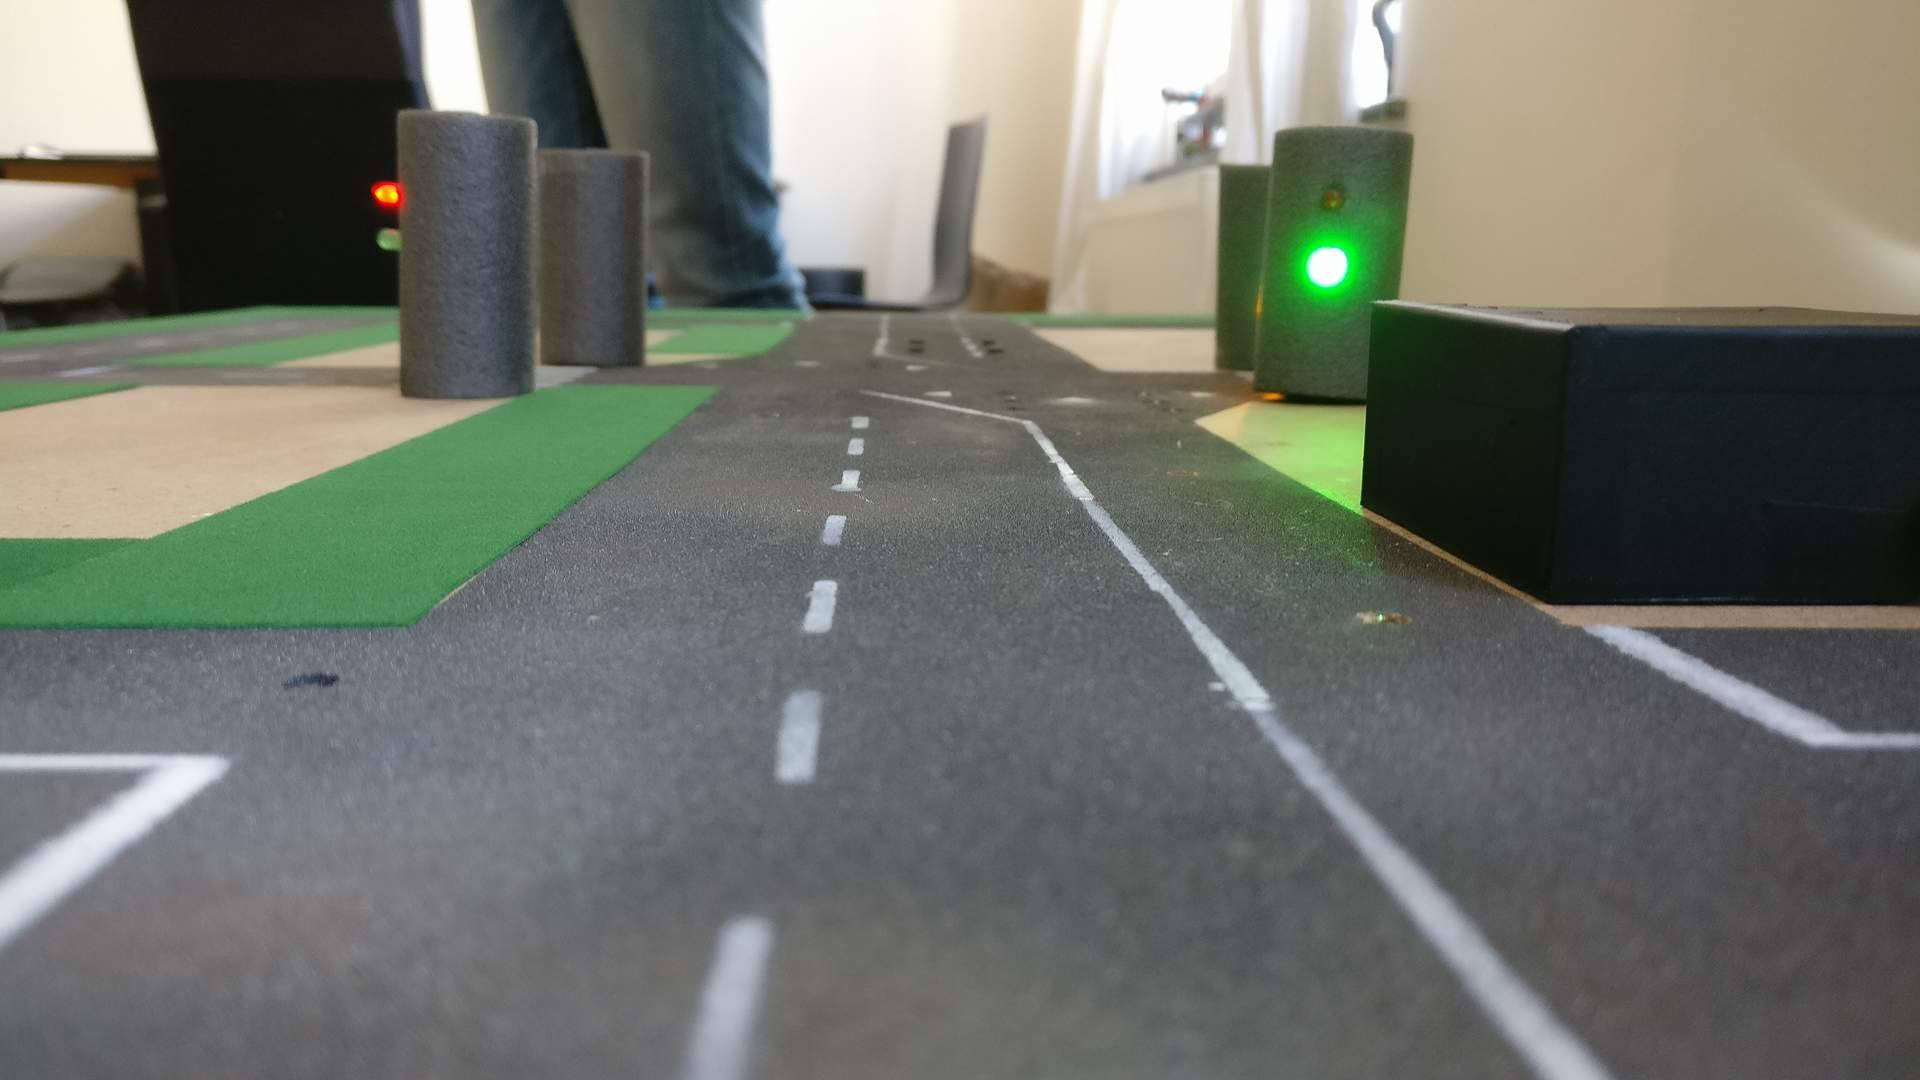
\includegraphics[width=\linewidth, height=\textheight,keepaspectratio]{img/maquette_1}}
        \caption{Point de vue d'un automobiliste}
    \end{center}
\end{figure}

\begin{figure}[H]
    \begin{center}
        \frame{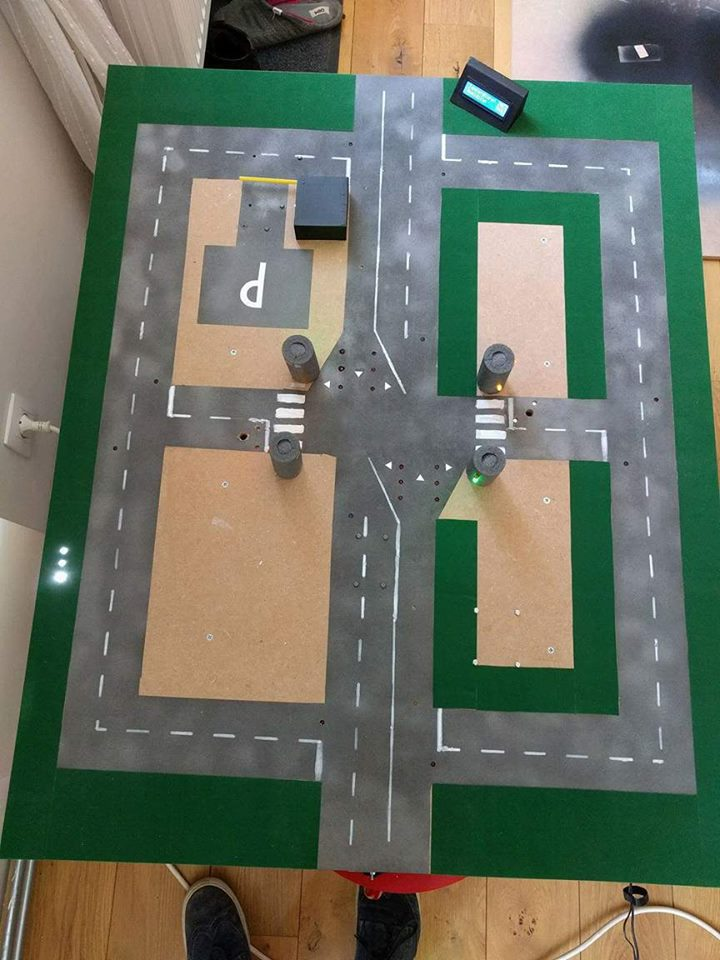
\includegraphics[width=\linewidth, height=\textheight,keepaspectratio]{img/maquette_2}}
        \caption{Maquette en cours de finalisation}
    \end{center}
\end{figure}

\begin{figure}[H]
    \begin{center}
        \frame{\includegraphics[width=\linewidth, height=\textheight,keepaspectratio]{img/maquette_3}}
        \caption{Maquette terminée}
    \end{center}
\end{figure}

\subsection{Code MySQL de la base de données}
\lstinputlisting[language=SQL, stepnumber=5, firstnumber=1, numberfirstline=true]{smartcity.sql}